\documentclass[a4paper,10pt]{article} % Default font size and paper size

\usepackage[T1]{fontenc}
\usepackage{multicol}
\usepackage{marvosym}
\usepackage{wasysym}
\usepackage{multirow}
\usepackage{blindtext}
\usepackage{polyglossia} 
\usepackage{xunicode,xltxtra,url,parskip}
\usepackage[usenames,dvipsnames]{xcolor}
\usepackage{enumitem}
\setitemize{noitemsep,topsep=0pt,parsep=1pt,partopsep=0pt}
\setlength{\textfloatsep}{-3cm}
\usepackage{marvosym}

\setlist{leftmargin=5mm}

\definecolor{grays}{rgb}{0.33, 0.33, 0.33}
\definecolor{grees}{rgb}{0.60, 0.67, 0.12}
\definecolor{blue}{rgb}{0.085, 0.234, 0.4}
\setdefaultlanguage[spelling=modern]{russian}
\setotherlanguage{english}
\usepackage{fontspec}

\setmonofont{[cmuntt.otf]}
\newfontfamily\cyrillicfont[  
	BoldFont        = [cmunbx.otf],
    ItalicFont      = [cmunti.otf],
    BoldItalicFont  = [cmunbx.otf],
    SmallCapsFont   = [cmunrm.otf],
    Mapping         = tex-text
]{[cmunrm.otf]}

% Параметры страницы
\textheight=27cm
\textwidth=19.5cm
\oddsidemargin=-2mm
\evensidemargin=-5mm
\marginparwidth=36pt
\topmargin = -3cm
\footnotesep=3ex
\hoffset = -1.5cm
\tolerance 3000
% подавить эффект "висячих стpок"
\clubpenalty=10000
\widowpenalty=10000

\usepackage{hyperref} % Required for adding links	and customizing them
\definecolor{linkcolour}{rgb}{0,0.0,0.0} % Link color
\hypersetup{colorlinks,breaklinks,urlcolor=linkcolour,linkcolor=linkcolour} % Set link colors throughout the document

\usepackage{titlesec} % Used to customize the \section command
\titleformat{\section}{\Large\scshape\raggedright}{}{0em}{}[\titlerule] % Text formatting of sections
\titlespacing{\section}{0pt}{3pt}{3pt} % Spacing around sections
\title{ashuha_resume}

\begin{document}

\pagestyle{empty} % Removes page numbering

\font\fb=''[cmr10]'' % Change the font of the \LaTeX command under the skills section
\oddsidemargin=0pt 		% отступ от левого края
%----------------------------------------------------------------------------------------
%	NAME AND CONTACT INFORMATION
%----------------------------------------------------------------------------------------

\begin{center}
	{\huge Arsenii Ashukha}
\end{center}
\begin{center}
\textcolor{gray}{
Moscow \& Amsterdam $\bullet$ 
\Letter~\textcolor{gray}{\texttt{ars.ashuha@gmail.com}} $\bullet$ \href{https://ars-ashuha.ru/}{\textcolor{gray}{\texttt{ars-ashuha.ru}}} $\bullet$
23 years old} 

\end{center}
\setlength{\columnsep}{-330pt}
\begin{multicols}{2}
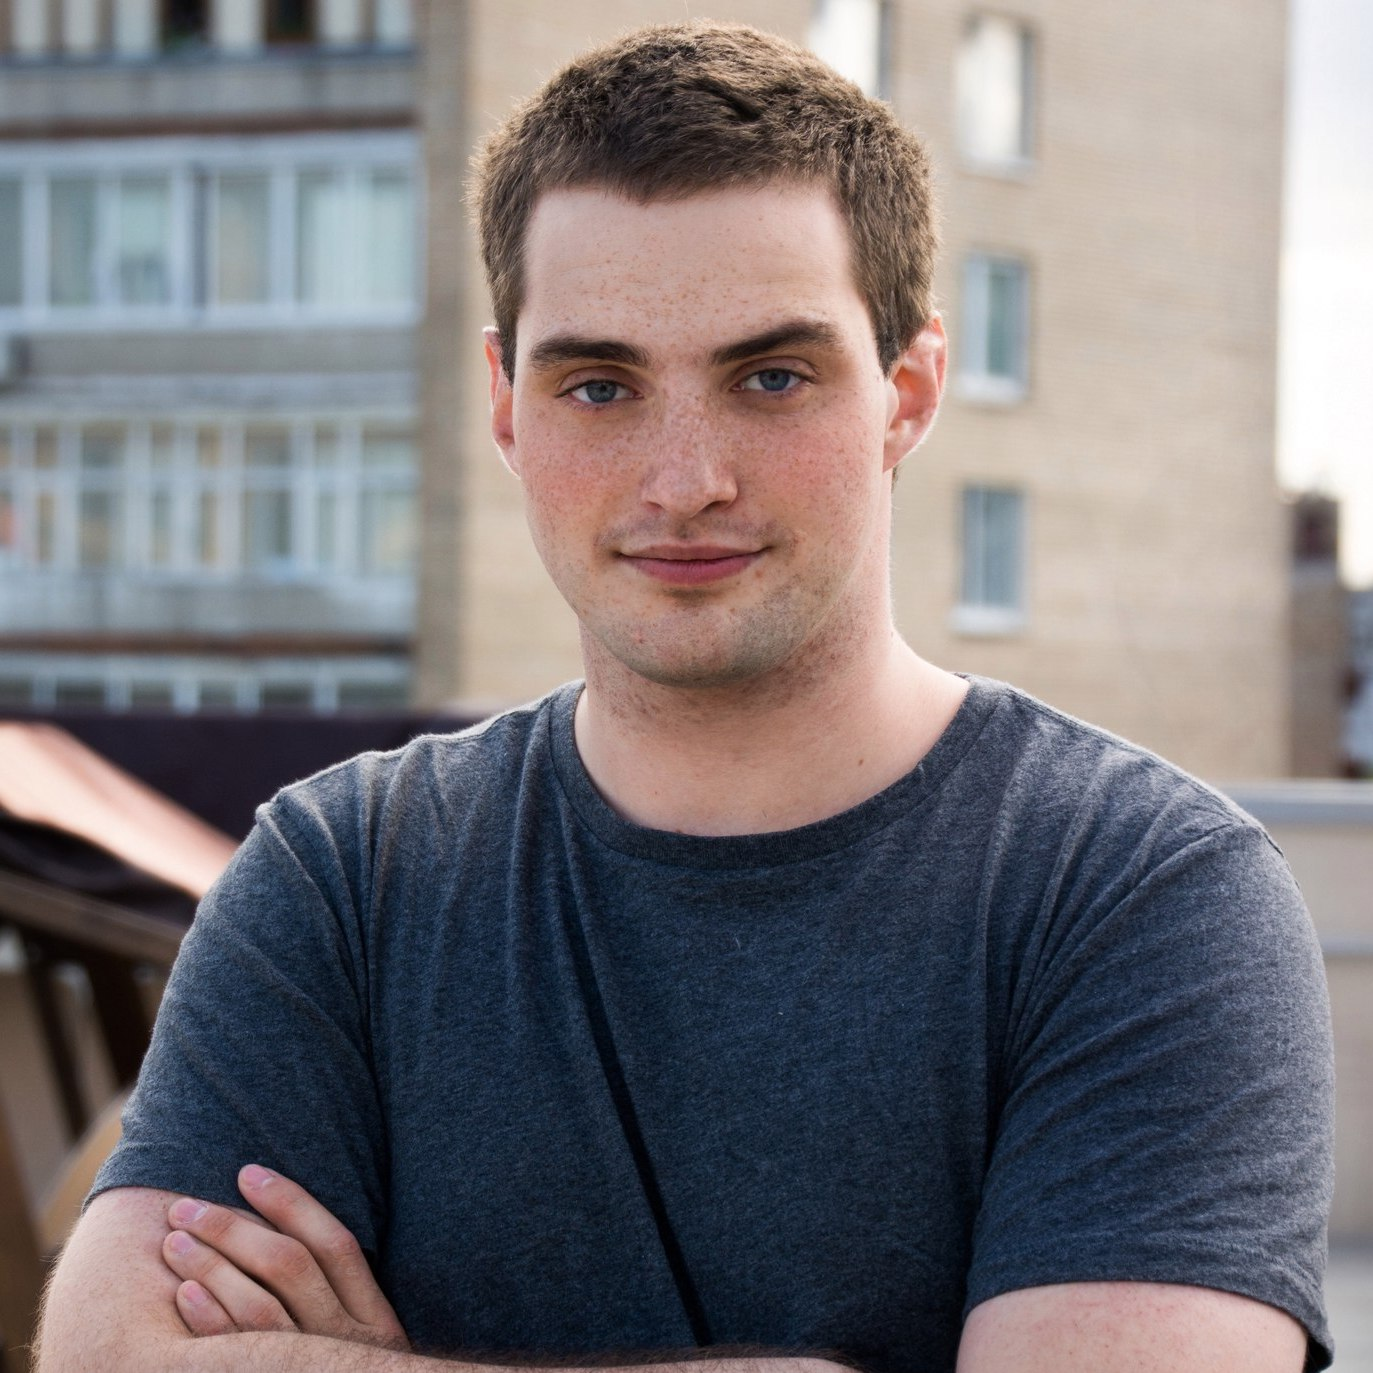
\includegraphics[scale=0.07]{../images/avatar_v3}

\section{Summary}
 \vspace{-0.2cm}
I'm getting PhD at University of Amsterdam jointly with Yandex Research, focused on Bayesian Deep Learning by supervision of Dmitry Vetrov and Max Welling.
Also, I teach several scientific seminars on Machine Learning and involved in research at HSE. 
My publications are available at \href{https://scholar.google.com/citations?user=IU-kuP8AAAAJ&hl=en}{\texttt{\textcolor{blue}{Google\,Scholar}}}.

\vspace{0.2cm}
\textbf{Skills}: Machine Learning, Deep Learning, Bayesian ML, Python, Linux, Fluent English

\end{multicols}

%----------------------------------------------------------------------------------------
%	EDUCATION
%----------------------------------------------------------------------------------------

\section{Education}

\begin{tabular}{rp{14cm}c}	
	\textbf{2017 -  2021} & PhD Candidate, \emph{Machine Learning}, \href{https://mipt.ru/english}{University of Amsterdam and Yandex Research} & \multirow{2}{*}{
\includegraphics[scale=0.015]{img/uva}}\\
	\textsc{Working on} & \emph{Bayesian Deep Learning} by supervision of \href{https://www.hse.ru/en/staff/dvetrov}{Dmitry Vetrov (\texttt{\textbf{Yandex}})} and \href{https://staff.fnwi.uva.nl/m.welling/}{Max Welling (\texttt{\textbf{UvA}})}
\end{tabular}

\begin{tabular}{rp{14cm}c}	
	\textbf{2015 -  2017} & Master, \emph{Machine Learning}, \href{https://mipt.ru/english}{Moscow Institute of Physics and Technology}, GPA: 4.8/5.0& \multirow{2}{*}{
\includegraphics[scale=0.15]{img/mipt}}\\
	\textsc{Thesis} & \emph{Variational Dropout Sparsifies DNNs}, Supervisor: \href{https://www.hse.ru/en/staff/dvetrov}{Dmitry Vetrov (\texttt{\textbf{HSE}})}, \href{https://ru.linkedin.com/in/alexey-dral}{Alex Dral (\texttt{\textbf{MIPT}})}
\end{tabular}

\begin{tabular}{rp{14cm}c}	
	\textbf{2015 -  2016} & Irregular Student, \emph{Machine Learning}, \href{https://yandexdataschool.com/}{Yandex School of Data Analysis}, GPA: 4.8/5.0& \multirow{2}{*}{~~
\includegraphics[scale=0.25]{img/shad}}\\
	\textsc{Result}~& \emph{Six courses were passed and the favorites are Bayesian ML, Deep Learning, Machine Learning}
\end{tabular}

\begin{tabular}{rp{14cm}c}	
\textbf{2011 -  2015} & Bachelor, \emph{Computer Science}, \href{http://www.bmstu.ru/en/}{Bauman Moscow State Technical University}, GPA: 3.7/5.0 & \multirow{2}{*}{~~~~~
\includegraphics[scale=0.012]{img/bmstu}}\\
\textsc{Thesis} &\emph{\href{https://github.com/ars-ashuha/bigram-anchor-words}{\textcolor{black}{Building of Uncorrelated Kernels for Topic Models}}}, Supervisor:  \href{https://scholar.google.ru/citations?user=FKkWXLkAAAAJ&hl=en}{\textcolor{black}{N. Loukachevitch~(\texttt{\textbf{MSU}})}}
\end{tabular}



\section{Experience}


\begin{tabular}{l|p{11.5cm}c}
\textbf{Sep 2017~ - nowadays} & 
\textbf{Yandex}, Moscow --- Researcher at Applied Research Team&
\multirow{2}{*}{	\vspace*{+5cm}
\includegraphics[scale=0.014]{img/yandex}} \\
~~~~~~~~~~~&  
\footnotesize{  \vspace{-0.25cm}
	\scriptsize{
		\emph{Chief}: 
		Dmitriy Vetrov
		(\href{mailto:vetrovd@yandex.ru}{\textcolor{gray}{vetrovd@yandex.ru}}),
	Pavel Serdyukov
	(\href{mailto:pavser@yandex-team.ru}{\textcolor{gray}{pavser@yandex-team.ru}})}
	\vspace{-0.1cm}} & 
\\
\multicolumn{2}{c}{}\\

\textbf{Mar 2017 - nowadays} & 
\textbf{HSE}, Moscow --- Intern Researcher at Bayesian Deep Learning Lab &
\multirow{2}{*}{	\vspace*{+5cm}
\includegraphics[scale=0.03]{img/hse}} \\
~~~~~~~~~~~&  
\footnotesize{  \vspace{-0.25cm}
\scriptsize{
	\emph{Chief}: 
	Dmitriy Vetrov
	(\href{mailto:vetrovd@yandex.ru}{\textcolor{gray}{vetrovd@yandex.ru}})}
	\vspace{-0.1cm}} & 
\\
\multicolumn{2}{c}{}\\


\textbf{Jun 2016 - Aug 2016} & 
\textbf{Yandex}, Moscow --- Intern at Music Deep Learning Group &
\multirow{2}{*}{
\includegraphics[scale=0.014]{img/yandex}} \\ 
\textcolor{gray}{3 months}~~~~~~~~~~~&  \footnotesize{
  
  \vspace{-0.25cm}
  \begin{itemize}
      \item[-] The quality of searching similar tracks and recommendation using DNN has been improved
      \item[-] Similar tracks system is working in production at \url{music.yandex.ru} 
  \end{itemize}
\scriptsize{
	\emph{Chief}:  
	Eugene Krofto
	(\href{mailto:singleton@yandex-team.ru}{\textcolor{gray}{singleton@yandex-team.ru}})}
  \vspace{-0.1cm}
} & 
\\
\multicolumn{2}{c}{}\\

\textbf{Dec 2013 - Feb 2016} &  
\textbf{Rambler}, Moscow --- R\&D Engineer at Machine Learning Group  &
\multirow{1}{*}{
\includegraphics[scale=0.1]{img/ramblerco}}\\ 
\textcolor{gray}{2 years part time}~~ &  \footnotesize{
  \vspace{-0.25cm}
  \begin{itemize}
      \item[-] The quality and the performance of user classification using url-history has been improved
  	  \item[-] Has been developed recommendations system for a news posts on \texttt{rambler.ru}
  \end{itemize}
	\scriptsize{
	\emph{Chief}:  
	\href{https://ru.linkedin.com/in/pavel-klemenkov-7a88a956}{Pavel Klemenkov} 
	(\href{mailto:pklemenkov@gmail.com}{\textcolor{gray}{pklemenkov@gmail.com}}),
	\href{https://ru.linkedin.com/in/anton-gorokhov-2959482}{Anton Gorokhov}
	(\href{mailto:anton.gorokhov@gmail.com}{\textcolor{gray}{anton.gorokhov@gmail.com}})}
  \vspace{-0.1cm}
} & 
\\
\multicolumn{2}{c}{}\\

\textbf{Jun 2013 - Aug 2013} & 
\textbf{Rambler}, Moscow --- Intern at Search Group&
\multirow{1}{*}{
\includegraphics[scale=0.1]{img/ramblerco}}\\ 
\textcolor{gray}{3 months}& 
\footnotesize{

\vspace{-0.25cm}
\begin{itemize}
	\item[-] Has been developed query clf system to use widgets in a web search result adaptively
\end{itemize}
\scriptsize{
	\emph{Chief}:  
Max Karpenko
(\href{mailto:v3dmax@gmail.com}{\textcolor{gray}{v3dmax@gmail.com}})}
\vspace{-0.1cm}
}& 
\\
\end{tabular}

\section{Teaching}
\begin{itemize}
	\item \textbf{Feb 2016 - Feb~\,2017:} Practical Lecturer of  \texttt{Machine Learning} at  MIPT {\small (}\href{https://ml-mipt.github.io}{\textcolor{blue}{page}}{\small )}
	\item  \textbf{Feb 2017 - Aug 2017:}  Lecturer of Deep Learning block in \texttt{Machine Learning} at MIPT
	{\small (}\href{https://ml-mipt.github.io/index-spring-2017/}{\textcolor{blue}{page}}{\small )}
	\item  \textbf{Oct 2016 - Aug 2017:}  Lecturer of Deep Learning block in \href{https://vk.com/data_mining_in_action}{\texttt{Data Mining in Action}}
	{\small (}\href{https://vk.com/data_mining_in_action}{\textcolor{blue}{page}},
	\href{https://www.youtube.com/channel/UCop3CelRVvrchG5lsPyxvHg}{\textcolor{blue}{video}}{\small )}
	
	\item  \textbf{Feb 2017 - nowadays:} Supervisor of \texttt{Scientific seminar on Machine Learning} at 
	HSE {\small (}\href{https://goo.gl/xuuRWx}{\textcolor{blue}{page}{\small)}} and 
	YSDA  {\small (}\href{https://yandexdataschool.com}{\textcolor{blue}{page}{\small)}} 
\end{itemize}

\end{document}

